
\section{A game-semantic account of safety}
\label{sec:gamesemaccount} Our aim is to characterize safety by game
semantics. We shall assume that the reader is familiar with the
basics of game semantics; For an introduction, we recommend
\cite{abramsky:game-semantics-tutorial}. Recall that a
\emph{justified sequence} over an arena is an alternating sequence
of O-moves and P-moves such that every move $m$, except the opening
move, has a pointer to some earlier occurrence of the move $m_0$
such that $m_0$ enables $m$ in the arena. A \emph{play} is just a
justified sequence that satisfies Visibility and Well-Bracketing. A
basic result in game semantics is that $\lambda$-terms are denoted
by \emph{innocent strategies}, which are strategies that depend only
on the \emph{P-view} of a play. The main result
(Theorem~\ref{thm:safeincrejust}) of this section is that if a
$\lambda$-term is safe, then its game semantics (is an innocent
strategy that) is, what we call, \emph{P-incrementally justified}. In such a
strategy, pointers emanating from the P-moves of a play are uniquely
reconstructible from the underlying sequence of moves and pointers
from the O-moves therein: specifically a P-question always points to
the last pending O-question (in the P-view) of a greater order.

The proof of Theorem~\ref{thm:safeincrejust} depends on a
Correspondence Theorem (see the Appendix) that relates the strategy
denotation of a $\lambda$-term $M$ to the set of \emph{traversals}
over a souped-up abstract syntax tree of the $\eta$-long form of $M$.
In the language of game semantics, traversals are just (concrete
representations of) the \emph{uncovering} (in the sense of Hyland
and Ong \cite{hylandong_pcf}) of plays in the strategy denotation.

The useful transference technique between plays and traversals was
originally introduced by one of us \cite{OngLics2006} for studying
the decidability of monadic second-order theories of infinite structures generated by
higher-order grammars (in which the $\Sigma$-constants or terminal symbols are at most
order 1, and \emph{uninterpreted}).
% In this setting, free variables are interpreted
% as constructors and therefore they do not have the ``full power'' of
% true free variables and are limited to order $1$ at most. Also,
% although the grammar can perform higher-order computations, the
% structure being studied is itself of ground type.
In the Appendix, we present an extension of this framework to the
general case of the simply-typed lambda calculus with free variables
of any order. A new traversal rule is introduced to handle nodes
labelled with free variables. Also new nodes are added to the
computation tree to account for the answer moves of the game
semantics, thus enabling the framework to model languages with
interpreted constants such as \pcf~(by adding traversal rules to
handle constant nodes).

\subsection*{Incrementally-bound computation tree}
 In \cite{OngLics2006} the computation tree of a grammar is
defined as the unravelling of a finite graph representing the \emph{long
transform} of a grammar. Similarly we define the computation tree of
a $\lambda$-term as an abstract syntax tree of its $\eta$-long
normal form.  We write $l\langle t_1, \ldots, t_n \rangle$ with $n
\geq 0$ to denote the ordered tree with a root labelled $l$ with $n$
child-subtrees $t_1$, \ldots, $t_n$. In the following we consider arbitrary
simply-typed terms.

\begin{definition}\rm
\label{dfn:comptree}
  The \defname{computation tree} $\tau(M)$ of a simply-typed term
  $\Gamma \stentail M:T$ with variable names in a countable set
  $\mathcal{V}$ is a tree with labels in $$ \{ @ \} \union \mathcal{V}
  \union \{ \lambda x_1 \ldots x_n \ | \ x_1 ,\ldots, x_n \in
  \mathcal{V}, n\in\nat \}$$ defined from its $\eta$-long form as follows. Suppose $\overline{x} = x_1 \ldots x_n$ for $n\geq 0$ then
\begin{eqnarray*}
  \mbox{for $m\geq 0$, $z \in \mathcal{V}$: } \tau(\lambda \overline{x} . z s_1 \ldots s_m : o) &=& \lambda \overline{x} \langle z \langle\tau(s_1),\ldots,\tau(s_m)\rangle\rangle \\
  \mbox{for $m \geq 1$: } \tau(\lambda \overline{x} . (\lambda y.t) s_1 \ldots s_m :o) &=& \lambda \overline{x} \langle @ \langle \tau(\lambda y.t),\tau(s_1),\ldots,\tau(s_m) \rangle \rangle \ .
\end{eqnarray*}
\end{definition}


Even-level nodes are $\lambda$-nodes (the root is on level 0). A
single $\lambda$-node can represent several consecutive variable
abstractions or it can just be a \emph{dummy lambda} if the
corresponding subterm is of ground type.  Odd-level nodes are
variable or application nodes.

The \defname{order} of a node $n$, written $\ord{n}$, is defined as
follows: @-nodes have order $0$. The order of a variable-node is the
type-order of the variable labelling it. The order of the root node
is the type-order of $(A_1,\ldots,A_p, T)$ where $A_1,\ldots, A_p$
are the types of the variables in the context $\Gamma$. Finally, the
order of a lambda node different from the root is the type-order of
the term represented by the sub-tree rooted at that node.

We say that a variable node $n$ labelled $x$ is \defname{bound} by a
node $m$, and $m$ is called the \defname{binder} of $n$, if $m$ is
the closest node in the path from $n$ to the root such that $m$ is
labelled $\lambda \overline{\xi}$ with $x\in \overline{\xi}$.


We introduce a class of computation trees in which the binder node
is uniquely determined by the nodes' orders:
\begin{definition}\rm
  A computation tree is \defname{incrementally-bound} if for all
  variable node $x$, either $x$ is \emph{bound} by the first
  $\lambda$-node in the path to the root with order $> \ord{x}$, or $x$
  is a \emph{free variable} and all the $\lambda$-nodes in the path to
  the root except the root have order $\leq \ord{x}$.
\end{definition}

\begin{proposition}[Safety and incremental-binding] \hfill
\label{prop:safe_imp_incrbound}
\begin{enumerate}[(i)]
\item If $M$ is safe then $\tau(M)$ is incrementally-bound.
\item Conversely, if $M$ is a \emph{closed} simply-typed term and $\tau(M)$
is incrementally-bound then $M$ is safe.
\end{enumerate}
\end{proposition}
\proof
  (i) Suppose that $M$ is safe. By Lemma
  \ref{prop:safe_iff_elnfsafe} the $\eta$-long form of $M$ is safe
  therefore $\tau(M)$ is the tree representation of a safe term.

In the safe lambda calculus, the variables in the context with the
lowest order must be all abstracted at once when using the
abstraction rule. Since the computation tree merges consecutive
abstractions into a single node, any variable $x$ occurring free in
the subtree rooted at a node $\lambda \overline{\xi}$ different from
the root must have order greater or equal to $\ord{\lambda
  \overline{\xi}}$. Conversely, if a lambda node $\lambda
\overline{\xi}$ binds a variable node $x$ then $\ord{\lambda
  \overline{\xi}} = 1+\max_{z\in\overline{\xi}} \ord{z} > \ord{x}$.

Let $x$ be a bound variable node. Its binder occurs in the path from
$x$ to the root, therefore, according to the previous observation,
$x$ must be bound by the first $\lambda$-node occurring in this path
with order $>\ord{x}$. Let $x$ be a free variable node then $x$ is
not bound by any of the $\lambda$-nodes occurring in the path to the
root. Once again, by the previous observation, all these
$\lambda$-nodes except the root have order smaller than $\ord{x}$.
Hence $\tau$ is incrementally-bound.

(ii) Let $M$ be a closed term such that $\tau(M)$ is
incrementally-bound.  W.l.o.g. we can assume that $M$ is in $\eta$-long
form.  We prove that $M$ is safe by induction on its structure. The
base case $M = \lambda \overline{\xi} . x$ for some variable $x$ is
trivial.  \emph{Step case:} If $M = \lambda \overline{\xi} . N_1
\ldots N_p$.  Let $i$ range over $1..p$. We have $N_i \equiv \lambda
\overline{\eta_i} . N'_i$ for some non-abstraction term $N'_i$. By
the induction hypothesis, $\lambda \overline{\xi} . N_i = \lambda
\overline{\xi} \overline{\eta_i} . N'_i$ is a safe closed term, and
consequently $N'_i$ is necessarily safe. Let $z$ be a free variable
of $N'_i$ not bound by $\lambda \overline{\eta_i}$ in $N_i$. Since
$\tau(M)$ is incrementally-bound we have $\ord{z} \geq \ord{\lambda
  \overline{\eta_1}} = \ord{N_i}$, thus we can abstract the variables $\overline{\eta_1}$ using \rulenamet{abs} which shows that $N_i$ is safe.  Finally
we conclude $\sentail M = \lambda \overline{\xi} . N_1 \ldots N_p :
T$ using the rules \rulenamet{app} and \rulenamet{abs}.  \qed



The assumption that $M$ is closed is necessary. For instance for
$x,y:o$, the computation trees $\tau(\lambda x y .x)$ and
$\tau(\lambda y . x)$ are both incrementally-bound but $\lambda x y
.x$ is safe and $\lambda y . x$ is not.

\subsection*{P-incrementally justified strategy}

We now consider the game-semantic model of the simply-typed lambda
calculus. The strategy denotation of a term-in-context $\Gamma
\stentail M : T$ is written $\sem{\Gamma
\stentail M : T}$. We define the \defname{order} of a move $m$,
written $\ord{m}$, to be the length of the path from $m$ to its
furthest leaf in the arena minus 1. (There are several ways to
define the order of a move; the definition chosen here is sound in
the current setting where each question move in the arena enables at
least one answer move.)
%{\it i.e.}~height of the subarena rooted at $q$ minus 2.

\begin{definition}\rm
  A strategy $\sigma$ is said to be \defname{P-incrementally
    justified} if for any play $s \, q \in \sigma$ where $q$ is a
  P-question, $q$ points to the last unanswered O-question in $\pview{s}$ with
  order strictly greater than $\ord{q}$.
\end{definition}
Note that although the pointer is determined by the P-view, the
choice of the move itself can be based on the whole history of the
play. Thus P-incremental justification does not imply innocence.

The definition suggests an algorithm that, given a play of a
P-incrementally justified denotation, uniquely recovers the pointers
from the underlying sequence of moves and from the pointers
associated to the O-moves therein. Hence:
\begin{lemma}
\label{lem:incrjustified_pointers_uniqu_recover} In P-incrementally
justified strategies, pointers emanating from P-moves are
superfluous.
\end{lemma}

\begin{example}
Copycat strategies, such as the identity strategy $id_A$ on game $A$
or the evaluation map $ev_{A,B}$ of type $(A \Rightarrow B) \times A
\typear B$, are all P-incrementally justified.\footnote{In such
strategies, a P-move $m$ is justified as follows: either $m$ points
to the preceding move in the P-view or the preceding move is of
smaller order and $m$ is justified by the second last O-move in the
P-view.}
\end{example}
%%%% the following example is wrong : ev is P-ij.
%
%\begin{example}
%Take the evaluation map $ev : (o^1 \Rightarrow o^2) \times o^3 \rightarrow o^4$ and the play $s = q^4 q^2 q^1 q^3 \in \sem{ev}$. We have $\ord{q^2} = 1 > \ord{q^1} = \ord{q^3} = 0$. Now $q^3$ points to $q^4$ but $q^2$ is the last unanswered O-question in $\pview{s}= s$ with order $>\ord{q^3}$, hence $\sem{ev}$ is not P-incrementally justified.
%\end{example}



The Correspondence Theorem~\ref{thm:correspondence}
% and Lemma \ref{lem:betanf_wellbehavedconst_trav_pview_red}
gives us the following equivalence:
\begin{proposition} % [Incremental-binding vs P-incremental justification]
\label{prop:Nher_incrbound_and_incrjustified} Let $\Gamma \stentail
M : T$ be a $\beta$-normal term. The computation tree $\tau(M)$ is
incrementally-bound if and only if $\sem{\Gamma \stentail M : T}$ is
P-incrementally justified.
\end{proposition}


\parpic[r]{
\raisebox{-12pt}
{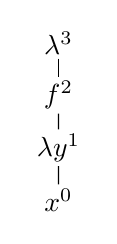
\begin{tikzpicture}[baseline=(root.base),level distance=4.4ex,inner ysep=0.5mm]
\node (root) {$\lambda^3$}
child {node {$f^2$}
       child {node {$\lambda y^1$}
              child {node {$x^0$}}}};
\end{tikzpicture}
}
}
%\noindent \emph{Example:}
\begin{example}
Consider the $\beta$-normal term $\Gamma\stentail f (\lambda y .x) :
o$ where $y:o$ and $\Gamma =f:((o,o),o),~x:o$. The figure on the
right represents its computation tree with the node orders given as
superscripts.  The node $x$ is not incrementally-bound therefore $\tau(f
(\lambda y .x))$ is not incrementally-bound and by Proposition
\ref{prop:Nher_incrbound_and_incrjustified}, $\sem{\Gamma \stentail
f (\lambda y .x) : o}$ is not incrementally-justified (although
$\sem{\Gamma \stentail f : ((o,o),o)}$ and $\sem{\Gamma \stentail
\lambda
  y. x : (o,o)}$ are).
\end{example}
\smallskip

Propositions \ref{prop:safe_imp_incrbound} and
\ref{prop:Nher_incrbound_and_incrjustified} allow us to show the
following:
\begin{theorem}[Safety and P-incremental justification]
\label{thm:safeincrejust} \hfill
\begin{enumerate}[(i)]
\item If $\Gamma \sentail M : T$ then $\sem{\Gamma \sentail M : T}$ is P-incrementally justified.
\item If $\stentail M : T$ is a closed simply-typed term and $\sem{\stentail M : T}$ is P-incrementally justified then the $\beta$-normal form of $M$ is safe.
\end{enumerate}
\end{theorem}
\proof (i) Let $M$ be a safe simply-typed term. By Lemma
\ref{lem:safered_preserve_safety}, its $\beta$-normal form $M'$ is
also safe. By Proposition \ref{prop:safe_imp_incrbound}(i),
$\tau(M')$ is incrementally-bound and by Proposition
\ref{prop:Nher_incrbound_and_incrjustified}, $\sem{M'}$ is an
incrementally-justified. Finally the soundness of the game model
gives $\sem{M} = \sem{M'}$.  (ii) is a consequence of Lemma
\ref{lem:safered_preserve_safety}, Proposition
\ref{prop:Nher_incrbound_and_incrjustified} and
\ref{prop:safe_imp_incrbound}(ii) and soundness of the game model.
\qed



Putting Theorem \ref{thm:safeincrejust}(i) and Lemma
\ref{lem:incrjustified_pointers_uniqu_recover} together gives:
\begin{proposition}
  \label{prop:safe_ptr_recoverable} In the game semantics of safe
  $\lambda$-terms, pointers emanating from P-moves are unnecessary
  {\it i.e.}~they are uniquely recoverable from the underlying sequences of
  moves and from O-moves' pointers.
\end{proposition}

% \begin{example} If justification pointers are omitted, the two
%   Kierstead terms from Example~\ref{ex:kierstead} have the same
%   denotation. In the safe lambda calculus the ambiguity disappears
%   since $M_1$ is safe whereas $M_2$ is not.
% \end{example}

In fact, as the last example highlights, pointers are superfluous at
order $3$ for safe terms whether from P-moves or O-moves. This is
because for question moves in the first two levels of an arena
(initial moves being at level $0$), the associated pointers are
uniquely recoverable thanks to the visibility condition. At the
third level, the question moves are all P-moves therefore their
associated pointers are uniquely recoverable by P-incremental
justification. This is not true anymore at order $4$: Take the safe
term $\psi:(((o^4,o^3),o^2),o^1) \sentail \psi (\lambda \varphi .
\varphi a) : o^0$ for some constant $a:o$, where $\varphi:(o,o)$.
Its strategy denotation contains plays whose underlying sequence of
moves is $q_0 \, q_1 \, q_2 \, q_3 \, q_2 \, q_3 \, q_4$. Since
$q_4$ is an O-move, it is not constrained by P-incremental
justification and thus it can point to any of the two occurrences of
$q_3$.\footnote{More generally, a P-incrementally justified strategy
can contain plays that are not ``O-incrementally justified'' since
it must take into account any possible strategy incarnating its
context, including those that are not P-incrementally justified. For
instance in the given example, there is one version of the play that
is not O-incrementally justified (the one where $q_4$ points to the
first occurrence of $q_3$). This play is involved in the strategy
composition $\sem{ \stentail M_2 : (((o,o),o),o)} ; \sem{
\psi:(((o,o),o),o) \stentail \psi (\lambda \varphi . \varphi a):o}$
where $M_2$ denotes the unsafe Kierstead term.}


\subsection*{Towards a fully abstract game model}\hfill

The standard game models which have been shown to be fully abstract
for PCF \cite{abramsky94full,hylandong_pcf} are of course also fully
abstract for the restricted language safe PCF. One may ask, however,
whether there exists a fully abstract model with respect to safe
context only. Such model may be obtain by considering
P-incrementally justified strategies. Its is reasonable to think
that O-moves also needs to be constrained by the symmetrical
O-incremental justification, which corresponds to the requirement
that contexts are safe. These issues will be addressed in Chapter
\ref{chap:model}.


\subsection*{Safe PCF and safe Idealised Algol}

\pcf\ is the simply-typed lambda calculus augmented with basic
arithmetic operators, if-then-else branching and a family of
recursion combinator $Y_A : ((A,A),A)$ for any type $A$.  We define
\emph{safe} \pcf\ to be \pcf\ where the application and abstraction
rules are constrained in the same way as the safe lambda calculus.
This language inherits the good properties of the safe lambda
calculus: No variable capture occurs when performing substitution
and safety is preserved by the reduction rules of the small-step
semantics of \pcf.

\subsubsection{Correspondence}

The computation tree of a \pcf\ term is defined as the least
upper-bound of the chain of computation trees of its \emph{syntactic
approximants} \cite{abramsky:game-semantics-tutorial}.  It is
obtained by infinitely expanding the $Y$ combinator, for instance
$\tau(Y (\lambda f x. f x))$ is the tree representation of the
$\eta$-long form of the infinite term $(\lambda f x. f x)
 ((\lambda f x. f x) ((\lambda f x. f x) ( \ldots$

It is straightforward to define the traversal rules modeling the
arithmetic constants of \pcf. Just as in the safe lambda calculus we
had to remove @-nodes in order to reveal the game-semantic
correspondence, in safe \pcf\ it is necessary to filter out the
constant nodes from the traversals. The Correspondence Theorem for
\pcf\ says that the interaction game semantics is isomorphic to the
set of traversals disposed of these superfluous nodes. This can
easily be shown for term approximants. It is then lifted to full
\pcf\ using the continuity of the function $\travset(\_)^{\filter
\theroot}$ from the set of computation trees (ordered by the
approximation ordering) to the set of sets of justified sequences of
nodes (ordered by subset inclusion). Finally computation trees of
safe \pcf\ terms are incrementally-bound thus we have
%Computation trees of safe \pcf\ terms are incrementally-bound.
%Moreover since \pcf\ constant are of order $1$ at most, the constant
%traversal rules are all \emph{well-behaved} (Lemma
%\ref{lem:sigma_order1_are_wellbehaved}) hence Lemma
%\ref{lem:betanf_wellbehavedconst_trav_pview_red} (from the Appendix)
%still holds and the game-semantic analysis of safety remains valid
%for \pcf. Hence we have:
\begin{theorem}
\label{thm:safepcfpincr} Safe PCF terms have P-incrementally
justified denotations. \qed
\end{theorem}


Similarly, we can define safe \ialgol\ to be safe \pcf\ augmented
with the imperative features of Idealized Algol (\ialgol\ for short)
\cite{Reynolds81}.  Adapting the game-semantic correspondence and
safety characterization to \ialgol\ seems feasible although the
presence of the base type \iavar, whose game arena $\iacom^{\nat}
\times \iaexp$ has infinitely many initial moves, causes a mismatch
between the simple tree representation of the term and its game
arena. It may be possible to overcome this problem by replacing the
notion of computation tree by a ``computation directed acyclic
graph''.

The possibility of representing plays \emph{without some or all of
  their pointers} under the safety assumption suggests potential
applications in algorithmic game semantics. Ghica and McCusker
\cite{ghicamccusker00} were the first to observe that pointers are
unnecessary for representing plays in the game semantics of the
second-order finitary fragment of Idealized Algol ($\ialgol_2$ for
short). Consequently observational equivalence for this fragment can
be reduced to the problem of equivalence of regular expressions.  At
order $3$, although pointers are necessary, deciding observational
equivalence of $\ialgol_3$ is EXPTIME-complete
\cite{DBLP:journals/apal/Ong04,DBLP:conf/fossacs/MurawskiW05}.
Restricting the problem to the safe fragment of $\ialgol_3$ may lead
to a lower complexity.

% (note that it is unlikely to obtain the complexity PSPACE because the
% set of complete plays of the safe term $\lambda f^{(o,o),o} . f
% (\lambda x^o . x)$ is not regular \cite{DBLP:journals/apal/Ong04}).

% Murawski showed the undecidability of program equivalence in
% $\ialgol_i$ for $i\geq4$ by encoding Turing machine computations
% into a finitary $IA_4$ term \cite{murawski03program}. The term
% constructed being not safe, the proof cannot be transposed to the
% safe fragments. Hence the question remains of whether observational
% equivalence is decidable for the \emph{safe} fragments of these
% language.

%In \cite{Ong02}, one of us showed that observational equivalence for
% finitary second-order \ialgol\ with recursion ($\ialgol_2 + Y_1$) is
% undecidable. The proof consists in reducing the Queue-Halting
% problem to the observational equivalence of two $\ialgol_2 + Y_1$
% terms. The same reduction is still valid in the safe fragment of
% $\ialgol_2 + Y_1$.  Consequently, observational equivalence of safe
% $\ialgol_2 + Y_1$ is also undecidable.
